% Copyright Sumin Yoo. Paper text: CC BY 4.0.
% Mathematical/software provenance and upstream MIT notice: SOURCES.md, NOTICE.
% This draft does not claim a completed non-Rupert proof.
\documentclass[11pt]{amsart}
\usepackage[T1]{fontenc}
\usepackage{lmodern,amsmath,amssymb,amsthm,booktabs,array}
\usepackage[margin=28mm]{geometry}
\usepackage{tikz,xcolor,xurl,hyperref}
\usetikzlibrary{arrows.meta,positioning}
\hypersetup{hidelinks,pdftitle={Towards a computer-assisted exclusion of Rupert's property for Johnson solid J73},pdfauthor={Sumin Yoo}}
\setlength{\emergencystretch}{2em}
\newcommand{\authorconfirm}[1]{\textnormal{\sffamily[AUTHOR-CONFIRM: #1]}}
\newcommand{\R}{\mathbb R}
\newcommand{\Q}{\mathbb Q}
\newcommand{\SO}{\operatorname{SO}}
\newcommand{\conv}{\operatorname{conv}}
\newcommand{\intr}{\operatorname{int}}
\newcommand{\diag}{\operatorname{diag}}
\newcommand{\tr}{\operatorname{tr}}
\newcommand{\ang}{\operatorname{ang}}
\newcommand{\proj}{\operatorname{proj}}
\newcommand{\norm}[1]{\lVert#1\rVert}
\newcommand{\cross}[1]{[#1]_\times}
\newcommand{\ip}[2]{\langle#1,#2\rangle}
\newcommand{\file}[1]{\path{#1}}
\newtheorem{theorem}{Theorem}[section]
\newtheorem{lemma}[theorem]{Lemma}
\newtheorem{proposition}[theorem]{Proposition}
\newtheorem{corollary}[theorem]{Corollary}
\theoremstyle{definition}
\newtheorem{definition}[theorem]{Definition}
\theoremstyle{remark}
\newtheorem{remark}[theorem]{Remark}
\title[J73: coincidence and exclusion certificates]{Towards a computer-assisted exclusion of Rupert's property\newline for the parabigyrate rhombicosidodecahedron}
\author{Sumin Yoo}
\address{Independent researcher, Republic of Korea}
\date{Interim report, version 0.1\\28 October 2026}
\begin{document}
\raggedbottom
\begin{abstract}
We study Rupert's property for the parabigyrate rhombicosidodecahedron,
Johnson solid J73. We exhibit an order-three symmetry $T$ of the parent
rhombicosidodecahedron such that $TP\ne P$ but the projections of $P$
and $TP$ agree on an open set of viewing directions. The two vertex sets
have forty points in common. Any box meeting this two-parameter family
contains a pose with zero separation margin. We give a uniform contact-patch theorem,
an exact signed-contact test, and a mixed first- and second-order tube
estimate near an intersection of coincidence families. These estimates
provide local exclusion criteria for a finite cover of the five-dimensional
configuration space. The computation and verification of the complete
cover are unfinished, so this report does not establish that J73 lacks
Rupert's property.
\end{abstract}
\maketitle

\noindent\emph{Status of this version.}
The local results are proved below. Production continues, and neither a
complete exclusion cover nor its exhaustive independent verification is
available. Table~\ref{tab:status} separates these obligations.

\begin{table}[ht]
\centering\small
\caption{Status at the time of this version.}
\label{tab:status}
\begin{tabular}{@{}p{.25\textwidth}p{.68\textwidth}@{}}
\toprule
Status & Scope\\
\midrule
Proved & Translation and symmetry reduction; the open coincidence
sheet; the contact-patch, signed-contact, mixed-tube, and membership
results under their stated hypotheses.\\
Computed, not yet fully verified & Production closures and replacement
trees in the frozen status snapshot; earlier retained certificates have
not all passed one exhaustive independent replay.\\
Open & A complete finite cover; conversion and independent checking of
the retained chain from every original root; the Rupert question for
J73. No completion date can be given.\\
\bottomrule
\end{tabular}
\end{table}

\section{Introduction}

A solid has Rupert's property if a congruent copy can pass through a
straight tunnel in it with positive clearance. For convex bodies the
problem can be expressed in terms of planar shadows: one asks whether an
orthogonal projection of one copy can be placed strictly inside an
orthogonal projection of the other. Contact alone does not give a passage.
This distinction matters when a numerical search approaches scale one.

The cube is Rupert, as are the other Platonic solids. Rupert's property
has also been established for many Archimedean and Johnson solids.
For the history of the problem, its projection formulation, and an
algorithmic approach, see Steininger and Yurkevich \cite{algorithmic,sy}.
Fredriksson used nonlinear optimization to find further passages
\cite{fredriksson}. Gosain and Grimmer later improved numerical passage
bounds \cite{gg}; Table~4 of their cited version lists no passage for
J72, J73, J74, J75, or J77.

Steininger and Yurkevich constructed the Noperthedron, a centrally
symmetric convex polyhedron with 90 vertices which does not have Rupert's
property \cite{sy}. Their proof combines global exclusion away from
contact with local arguments near the limiting configurations. Recent
preprints treat the two snub solids \cite{lw} and the
rhombicosidodecahedron \cite{jung,hervay}. Murphy has released Lean-based
verifications for the two snub solids \cite{murphy}; the kernel checks
conditional theorems, while compiled programs check the certificate data.
The present paper concerns J73.

We adapt Jung's computational framework to J73. The two opposite cupola
gyrations preserve central symmetry and leave a proper symmetry group
of order ten. An order-three rotation of the parent solid also preserves
certain shadows of J73, although it does not preserve the solid.
We describe this coincidence before giving the local certificates.

A complete finite exclusion cover would imply the following result.

\begin{theorem}[Conditional completion criterion]\label{thm:completion}
Let $P$ be the exact body in Section~\ref{sec:body}. Suppose the
certificate consists of a finite rooted forest of closed boxes whose
roots cover the reduced domain \eqref{eq:domain}. Every nonterminal node
has finitely many closed children whose union is exactly that node's box;
each replacement is bound to the identical parent region it replaces.
Suppose every reachable leaf has an exclusion certificate for its entire
box, using a proved local rule whose hypotheses and whole-box membership
are verified for $P$, with no unresolved or missing nodes. Then $P$ is
not Rupert.
\end{theorem}
\begin{proof}
By Lemma~\ref{lem:reduction}, a passage would give strict containment at
a point of the reduced domain. A root contains that point. At each
nonterminal node, at least one child contains it because the children
cover that node. The forest is finite and acyclic, so this process
terminates at a leaf containing the point,
also when it lies on a shared boundary. The verified rule for that box
excludes strict containment, a contradiction.
\end{proof}

The complete cover required by Theorem~\ref{thm:completion} has not yet
been verified.

\section{J73 and its symmetry reduction}\label{sec:body}

\subsection{Exact coordinates}
Put $s=\sqrt5$ and $\phi=(1+s)/2$. Let $V_0$ consist of the distinct signed
cyclic permutations of
\begin{equation}\label{eq:seeds}
 (1,1,\phi^3),\qquad (\phi^2,\phi,2\phi),\qquad
 (2+\phi,0,\phi^2),
\end{equation}
with independent signs on nonzero entries. Sort these sixty points
lexicographically in the real embedding of $\Q(s)$, retaining these
indices after the construction below. Put $a=(-\phi,-1,0)$ and
$h=\max_{v\in V_0}a\cdot v$. Define
\begin{equation}\label{eq:gyration}
 G=\frac\phi2 I+\frac{s-1}{4}\cross a
       +\left(\frac12-\frac{s}{5}\right)aa^{\mathsf T}.
\end{equation}
The matrix $G$ is a rotation through $\pi/5$ about the oriented axis $a$. Set
\begin{equation}\label{eq:body}
 p_i=\begin{cases}
 Gv_i,&a\cdot v_i=h,\\
 G^{\mathsf T}v_i,&a\cdot v_i=-h,\\
 v_i,&\text{otherwise},
 \end{cases}
 \qquad V=\{p_i:0\le i<60\},\quad P=\conv V.
\end{equation}
These are the edge-length-two body coordinates of J73. Only the five
vertices on each extreme pentagon change; the joining decagons are
permuted by the cupola rotations. Direct substitution gives
\begin{equation}\label{eq:bodychecks}
 V=-V,\qquad \norm{p_i}^2=R_b^2=11+4s.
\end{equation}
The input checker verifies that the vertices are distinct, that the 120
edges have squared length four, and that the symmetries below permute
$V$ \cite{input}. All certificate indices retain the parent ordering.

The vertices and reference rotations used in the exact contact identities
have entries in $\Q(s)$. The alignment matrix
\begin{equation}\label{eq:align}
 A=\begin{pmatrix}
 0&0&1\\
 -1/\sqrt{\phi+2}&\phi/\sqrt{\phi+2}&0\\
 -\phi/\sqrt{\phi+2}&-1/\sqrt{\phi+2}&0
 \end{pmatrix}
\end{equation}
belongs to $\SO(3)$ and maps $a$ to the positive vertical axis.
The pipeline uses the normalized vertices $Ap_i/R_b$, whose coordinates
require a larger algebraic field. We use $P$ in body coordinates for the local theorems; common
scaling does not change shadow containment.

\subsection{Proper symmetries and screen frames}
The rotations
\[
 D=\{G^{2k},SG^{2k}:0\le k<5\},\qquad S=\diag(-1,-1,1),
\]
preserve $V$. They satisfy $(G^2)^5=S^2=I$ and
$SG^2S=G^{-2}$, so $D\cong D_5$ has order ten. The reduction uses
only the verified subgroup $D$ and central symmetry. In aligned coordinates the subgroup is generated
by a vertical fifth-turn and a horizontal half-turn \cite{input}.

For $t,p\in\R$ write
\begin{equation}\label{eq:frame}
 F(t,p)=\begin{pmatrix}
 -\sin t&\cos t&0\\
 -\cos t\cos p&-\sin t\cos p&\sin p\\
 \cos t\sin p&\sin t\sin p&\cos p
 \end{pmatrix}\in\SO(3),
\end{equation}
and let $M(t,p)$ be its first two rows. With $R_2(\alpha)$ a positive
planar rotation, a configuration is
\[
 x=(t_i,p_i,t_o,p_o,\alpha),\quad
 K_i(x)=R_2(\alpha)M(t_i,p_i)AP,\quad K_o(x)=M(t_o,p_o)AP.
\]
Here $p_i,p_o$ denote polar angles, whereas $p_j$ denotes a body vertex.

\begin{lemma}[Translation and symmetry reduction]\label{lem:reduction}
The body $P$ is Rupert if and only if $K_i(x)\subset\intr K_o(x)$ for
some $x$ in the closed domain
\begin{equation}\label{eq:domain}
 \mathcal D=([0,2\pi/5]\times[0,\pi/2])^2
                         \times[-\pi/2,\pi/2].
\end{equation}
\end{lemma}
\begin{proof}
Let $K=-K$ and $L=-L$ be convex planar bodies. If
$K+t\subset\intr L$, then $K-t\subset\intr L$ as well. The midpoint of
$z+t$ and $z-t$ belongs to $\intr L$ for every $z\in K$, since the
interior is convex. Thus $K\subset\intr L$, and translations may be
removed.

Represent each spatial orientation by a proper frame. A half-turn in
the aligned dihedral group moves a lower-hemisphere view to the upper
hemisphere. A fifth-turn puts its azimuth in $[0,2\pi/5]$. Apply these
body symmetries independently to the two copies. Two proper frames with
the same third row differ by a proper screen rotation. A common screen
rotation removes the outer screen angle, leaving $\alpha$ as their
difference. Central symmetry makes this angle periodic modulo $\pi$.
This gives \eqref{eq:domain}. Poles and endpoints may have several
representatives, which causes no problem for a closed cover. Every
configuration in the stated domain is an allowed original configuration,
so the converse follows. The projection formulation of Rupert's property
then gives the result \cite{sy}.
\end{proof}

\section{The hidden coincidence}\label{sec:hidden}

\subsection{An order-three rotation}
Consider the proper rotation
\begin{equation}\label{eq:T}
 T=\frac14\begin{pmatrix}
 1+s&s-1&-2\\
 1-s&-2&-1-s\\
 -2&1+s&1-s
 \end{pmatrix}.
\end{equation}
It satisfies $T^{\mathsf T}T=I$, $\det T=1$, $T^3=I$, and $\tr T=0$.
It is therefore a rotation through $120$ degrees. It permutes $V_0$, but
\begin{equation}\label{eq:shared}
 |V\cap TV|=40,\qquad |V\cup TV|=80.
\end{equation}
In particular, it is not a J73 symmetry. Some earlier records use the
improper matrix $H=-T$. Since $P=-P$, we have $HP=TP$; throughout this
section we use $T\in\SO(3)$ \cite{hidden}.

Let $W=V\cup TV$, and take the cyclic index list
\begin{equation}\label{eq:cycle}
 (22,28,16,20,32,33,41,29,35,37,31,43,39,27,26,18,30,24).
\end{equation}
Writing it as $(i_0,\ldots,i_{17})$, with cyclic subscripts, define,
for $0\le j<18$, $z\in W$, and $w\in\R^3$,
\[
 N_{j,z}=(p_{i_{j+1}}-p_{i_j})\times(z-p_{i_j}),\qquad
 \mathcal C=\{w:w\cdot N_{j,z}>0\text{ whenever }N_{j,z}\ne0\}.
\]

\begin{proposition}[An open coincidence sheet]\label{prop:coincidence}
The cone $\mathcal C$ is nonempty and open. For every $w\in\mathcal C$,
the orthogonal projections of $P$ and $TP$ onto $w^\perp$ coincide and
have boundary cycle \eqref{eq:cycle}.
\end{proposition}
\begin{proof}
All eighteen listed vertices belong to $V\cap TV$. At
\[
 w_*={(-1007120,-93249,276631)}/{1048576},
\]
the $18\cdot80$ scalar products defining the cone have 1404 positive
values and 36 zeros. In every zero case $N_{j,z}=0$: these are the two
endpoints of each edge. The least positive value is
\[
 (-1470249+730489\sqrt5)/1048576>0.
\]
The discovery program reconstructs these scalar products from the stated
coordinates and boundary cycle, \eqref{eq:seeds}--\eqref{eq:cycle}, and
determines their signs exactly in $\Q(\sqrt5)$. The release run returned
1,404 positive values; the remaining 36 cases have $N_{j,z}=0$. For any $w$ in the cone, each listed edge is a supporting
edge of $\conv\proj_w W$, and every other projected point is on its
strict inner side. The projected cycle is consequently a convex
eighteen-gon containing $\proj_w W$. Its vertices belong to both shadows,
which proves equality. Finally, $\mathcal C$ is a finite intersection of
open linear half-spaces containing $w_*$. Its intersection with the sphere
is a nonempty open set of viewing directions.
\end{proof}

For each $w\in\mathcal C$, the largest scale allowed under non-strict
containment at relative rotation $T$ is one. Scale one is attained because
the shadows coincide, and no larger scale is possible because their areas
are equal. This conclusion concerns only the relative poses specified above.
More precisely, let
\[
 \lambda_T(w)=\sup\{r\ge0:\exists t\in w^\perp,
                   \ r\proj_w(TP)+t\subseteq\proj_wP\}.
\]
Then $\lambda_T(w)=1$ for $w\in\mathcal C$; this is not a
maximization over all pairs of orientations. A related distinction
between contact and passage occurs in the author's earlier study of a
touching arc of the snub cube \cite{yoo}. Here the coincidence directions
form an open subset of the sphere rather than an arc.

\begin{figure}[ht]
\centering
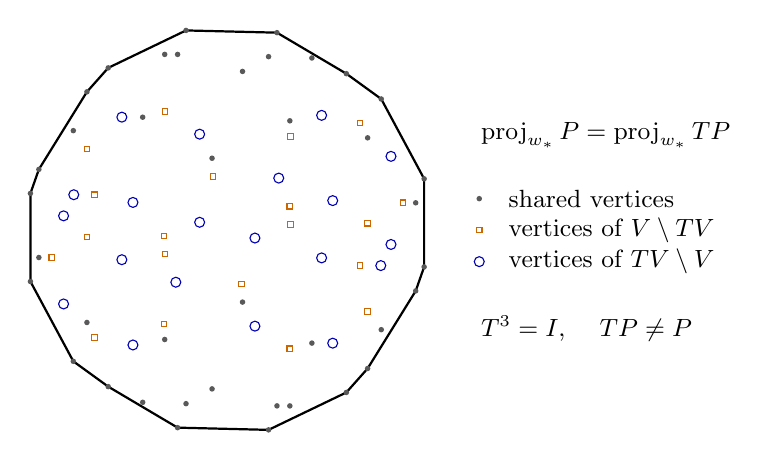
\begin{tikzpicture}[font=\small]
 \draw[thick] (-0.524056,2.536347)--(-1.511992,2.061051)--(-1.782404,1.756843)--(-2.392982,0.771573)--(-2.499929,0.466850)--(-2.499929,-0.652055)--(-1.955447,-1.665540)--(-1.511992,-1.987185)--(-0.631003,-2.508133)--(0.524056,-2.536347)--(1.511992,-2.061051)--(1.782404,-1.756843)--(2.392982,-0.771573)--(2.499929,-0.466850)--(2.499929,0.652055)--(1.955447,1.665540)--(1.511992,1.987185)--(0.631003,2.508133)--cycle;
 \fill[black!65] (0.193468,2.015915) circle (1pt);
 \fill[black!65] (0.193468,-0.913416) circle (1pt);
 \fill[black!65] (-0.794468,2.232139) circle (1pt);
 \fill[black!65] (-0.794468,-1.388712) circle (1pt);
 \fill[black!65] (1.074458,2.186488) circle (1pt);
 \fill[black!65] (1.074458,-1.434364) circle (1pt);
 \fill[black!65] (-1.782404,1.756843) circle (1pt);
 \fill[black!65] (-1.782404,-1.172487) circle (1pt);
 \fill[black!65] (1.955447,1.665540) circle (1pt);
 \fill[black!65] (1.955447,-1.263791) circle (1pt);
 \fill[black!65] (-2.392982,0.771573) circle (1pt);
 \fill[black!65] (-2.392982,-0.347332) circle (1pt);
 \fill[black!65] (-0.524056,2.536347) circle (1pt);
 \fill[black!65] (-0.524056,-2.203410) circle (1pt);
 \fill[black!65] (0.631003,2.508133) circle (1pt);
 \fill[black!65] (0.631003,-2.231624) circle (1pt);
 \fill[black!65] (2.499929,0.652055) circle (1pt);
 \fill[black!65] (2.499929,-0.466850) circle (1pt);
 \fill[black!65] (-1.511992,2.061051) circle (1pt);
 \fill[black!65] (-1.511992,-1.987185) circle (1pt);
 \fill[black!65] (1.511992,1.987185) circle (1pt);
 \fill[black!65] (1.511992,-2.061051) circle (1pt);
 \fill[black!65] (-2.499929,0.466850) circle (1pt);
 \fill[black!65] (-2.499929,-0.652055) circle (1pt);
 \fill[black!65] (-0.631003,2.231624) circle (1pt);
 \fill[black!65] (-0.631003,-2.508133) circle (1pt);
 \fill[black!65] (0.524056,2.203410) circle (1pt);
 \fill[black!65] (0.524056,-2.536347) circle (1pt);
 \fill[black!65] (2.392982,0.347332) circle (1pt);
 \fill[black!65] (2.392982,-0.771573) circle (1pt);
 \fill[black!65] (-1.955447,1.263791) circle (1pt);
 \fill[black!65] (-1.955447,-1.665540) circle (1pt);
 \fill[black!65] (1.782404,1.172487) circle (1pt);
 \fill[black!65] (1.782404,-1.756843) circle (1pt);
 \fill[black!65] (-1.074458,1.434364) circle (1pt);
 \fill[black!65] (-1.074458,-2.186488) circle (1pt);
 \fill[black!65] (0.794468,1.388712) circle (1pt);
 \fill[black!65] (0.794468,-2.232139) circle (1pt);
 \fill[black!65] (-0.193468,0.913416) circle (1pt);
 \fill[black!65] (-0.193468,-2.015915) circle (1pt);
 \draw[orange!80!black] (-0.792831,1.506804) ++(-.035,-.035) rectangle ++(.07,.07);
 \draw[orange!80!black] (-0.182253,0.681648) ++(-.035,-.035) rectangle ++(.07,.07);
 \draw[orange!80!black] (0.804046,1.190759) ++(-.035,-.035) rectangle ++(.07,.07);
 \draw[orange!80!black] (0.804046,0.071855) ++(-.035,-.035) rectangle ++(.07,.07);
 \draw[orange!80!black] (-1.780768,1.031508) ++(-.035,-.035) rectangle ++(.07,.07);
 \draw[orange!80!black] (-0.792831,-0.303622) ++(-.035,-.035) rectangle ++(.07,.07);
 \draw[orange!80!black] (1.685036,1.361332) ++(-.035,-.035) rectangle ++(.07,.07);
 \draw[orange!80!black] (1.685036,-0.449093) ++(-.035,-.035) rectangle ++(.07,.07);
 \draw[orange!80!black] (-1.780768,-0.087397) ++(-.035,-.035) rectangle ++(.07,.07);
 \draw[orange!80!black] (2.229517,0.347848) ++(-.035,-.035) rectangle ++(.07,.07);
 \draw[orange!80!black] (-2.229517,-0.347848) ++(-.035,-.035) rectangle ++(.07,.07);
 \draw[orange!80!black] (1.780768,-1.031508) ++(-.035,-.035) rectangle ++(.07,.07);
 \draw[orange!80!black] (-1.685036,0.449093) ++(-.035,-.035) rectangle ++(.07,.07);
 \draw[orange!80!black] (-1.685036,-1.361332) ++(-.035,-.035) rectangle ++(.07,.07);
 \draw[orange!80!black] (1.780768,0.087397) ++(-.035,-.035) rectangle ++(.07,.07);
 \draw[orange!80!black] (0.792831,-1.506804) ++(-.035,-.035) rectangle ++(.07,.07);
 \draw[orange!80!black] (-0.804046,-0.071855) ++(-.035,-.035) rectangle ++(.07,.07);
 \draw[orange!80!black] (-0.804046,-1.190759) ++(-.035,-.035) rectangle ++(.07,.07);
 \draw[orange!80!black] (0.792831,0.303622) ++(-.035,-.035) rectangle ++(.07,.07);
 \draw[orange!80!black] (0.182253,-0.681648) ++(-.035,-.035) rectangle ++(.07,.07);
 \draw[blue!70!black] (2.079026,-0.181679) circle (1.8pt);
 \draw[blue!70!black] (1.198037,-0.352252) circle (1.8pt);
 \draw[blue!70!black] (-0.351013,0.100069) circle (1.8pt);
 \draw[blue!70!black] (2.079026,0.937226) circle (1.8pt);
 \draw[blue!70!black] (0.653555,0.661232) circle (1.8pt);
 \draw[blue!70!black] (1.198037,1.458174) circle (1.8pt);
 \draw[blue!70!black] (-0.351013,1.218973) circle (1.8pt);
 \draw[blue!70!black] (-1.338949,-0.375228) circle (1.8pt);
 \draw[blue!70!black] (-1.338949,1.435198) circle (1.8pt);
 \draw[blue!70!black] (-1.949527,0.449928) circle (1.8pt);
 \draw[blue!70!black] (1.949527,-0.449928) circle (1.8pt);
 \draw[blue!70!black] (1.338949,-1.435198) circle (1.8pt);
 \draw[blue!70!black] (1.338949,0.375228) circle (1.8pt);
 \draw[blue!70!black] (0.351013,-1.218973) circle (1.8pt);
 \draw[blue!70!black] (-2.079026,-0.937226) circle (1.8pt);
 \draw[blue!70!black] (-1.198037,-1.458174) circle (1.8pt);
 \draw[blue!70!black] (-2.079026,0.181679) circle (1.8pt);
 \draw[blue!70!black] (0.351013,-0.100069) circle (1.8pt);
 \draw[blue!70!black] (-0.653555,-0.661232) circle (1.8pt);
 \draw[blue!70!black] (-1.198037,0.352252) circle (1.8pt);
 \node[anchor=west] at (3.1,1.2) {$\proj_{w_*}P=\proj_{w_*}TP$};
 \fill[black!65] (3.2,.4) circle (1pt);
 \node[anchor=west] at (3.45,.4) {shared vertices};
 \draw[orange!80!black] (3.165,-.035) rectangle ++(.07,.07);
 \node[anchor=west] at (3.45,0) {vertices of $V\setminus TV$};
 \draw[blue!70!black] (3.2,-.4) circle (1.8pt);
 \node[anchor=west] at (3.45,-.4) {vertices of $TV\setminus V$};
 \node[anchor=west] at (3.1,-1.25) {$T^3=I$, $\quad TP\ne P$};
\end{tikzpicture}
\caption{The common eighteen-edge shadow at $w_*$. The nonshared vertices
project inside it. The equality persists on an open set of views, by
Proposition~\ref{prop:coincidence}. Plot coordinates are rounded for display;
the proof uses the exact scalar products, not this drawing.}
\label{fig:hidden}
\end{figure}


\subsection{Fifty rotations and four hundred labels}
The double orbit
\begin{equation}\label{eq:orbit}
 \mathcal O=\{g_oTg_i^{\mathsf T}:g_o,g_i\in D\}
\end{equation}
contains fifty distinct rotations. Each has two representatives among
the one hundred ordered group pairs; none belongs to $D$. The exact
finite enumeration and vertex counts are supplied in \cite{hidden}.
If $U=g_oTg_i^{\mathsf T}$, then
\[
 \proj_{g_ow}(UP)=\proj_{g_ow}P\qquad(w\in\mathcal C).
\]
The corresponding inner view in its own body coordinates is
$g_iT^{\mathsf T}w$. An oriented pose record also retains a view sign
$\sigma\in\{-1,1\}$ and a screen lift
$L\in\{I,\diag(-1,-1,1)\}$. At the anchor the triples
\[
 (\sigma g_ow_*,\ g_oTg_i^{\mathsf T},\ L)
\]
give four hundred distinct labels. These labels record the viewing
direction and screen lift as well as the relative rotation; labels with
the same rotation may describe different view patches.

Any box meeting the coincidence sheet contains a pose with zero separation
margin. Exclusion near the sheet therefore requires an estimate that
permits equality on the sheet and controls nearby rotations.

At $w_*$ the discovery data also give four common contact vertices. Set
$(i_1,i_2,i_3,i_4)=(26,31,39,30)$ and $q_j=p_{i_j}$ for $1\le j\le4$.
Let $n_j\perp w_*$ be the uniquely supporting covector at $q_j$.
For the torques $b_j=q_j\times n_j$, the exact data give weights
$c_j>0$ with
\[
 \sum_j c_j=1,\qquad \sum_j c_jb_j=0,\qquad
                  \det(b_1,b_2,b_3)\ne0.
\]
For every nonzero infinitesimal rotation $\omega$, some
$b_j\cdot\omega$ is positive. Otherwise their positive weighted sum
would force all of them to vanish, contrary to the rank condition. This
is a fixed-view, first-order statement, not a uniform neighborhood
certificate. The included program \file{code/discovery/check.py} checks
these identities independently of production. Its reproduction record is
given with the frozen release data.

\section{Global and local certificates}\label{sec:certificates}

\subsection{Support differences}
For a compact convex body $K$, let $h_K(n)=\max_{q\in K}n\cdot q$.
For $w\ne0$ and $n\perp w$, this is also the support value of
$\proj_wK$. If $n\ne0$, $n\perp w$, and an inner point $q$ satisfies
$n\cdot q\ge h_P(n)$, then strict centered containment is impossible.
Central symmetry then
excludes translated strict containment by Lemma~\ref{lem:reduction}.
We first give a sufficient condition based on Taylor's formula.

\begin{lemma}[A global Taylor certificate]\label{lem:global}
Let $B=\prod_{d=1}^5[c_d-h_d,c_d+h_d]$. For a fixed inner vertex and
fixed nonzero planar covector $n$, put
$f_j(x)=n\cdot(z_i(x)-z_j^o(x))$, where $z_i,z_j^o$ are the inner and
outer projected vertices. Suppose verified bounds $M_{de,j}$ satisfy
$|\partial_d\partial_e f_j(x)|\le M_{de,j}$ on $B$ and, for every outer
vertex $j$,
\[
 f_j(c)-\sum_d|\partial_df_j(c)|h_d
       -\frac12\sum_{d,e}M_{de,j}h_dh_e\ge0.
\]
Then no configuration in $B$ gives strict shadow containment.
\end{lemma}
\begin{proof}
Taylor's formula along the segment from $c$ to $x$ gives the displayed
quantity as a lower bound for $f_j(x)$. Thus the inner point has support
value at least that of every outer vertex, for the same $n$.
\end{proof}

The release uses four certificate categories. $G$ checks a support
separation on the entire original angle box. $SC$ checks a nonnegative
weighted sum of exact contact differences. $COVER$ reconstructs closed
splits and coordinate covers. The $tube$ rule checks a certified local
region together with whole-box membership. These are the categories
implemented by the included independent checker; they are described in
Section~\ref{sec:interface}. Older production records use additional
labels, including $S$, $L2$, $L5$, balls, and collision witnesses. Their
presence in a historical producer record is not acceptance by the new
checker. Every retained witness must either be replayed under its original
proved rule or be converted and rechecked before it can contribute to a
complete independently verified cover.

\subsection{The contact-patch theorem}
The theorem allows any finite number of contacts. Our implementation
often uses four, but four contacts need not suffice.

\begin{theorem}[Uniform contact patch]\label{thm:patch}
Let $P=\conv V=-P$ be a full-dimensional polytope, with
$\norm q\le R_b$ for $q\in V$. Let $B$ be a closed polygon, and let
$w:B\to\R^3\setminus\{0\}$ be affine. Fix $U\in\SO(3)$ and pairs
$p_j,q_j\in V$ satisfying $Up_j=q_j$. Suppose affine covectors
$N_j(w)\perp w$ satisfy, on all of $B$,
\begin{align}
 N_j(w)\ne0,\qquad &N_j(w)\cdot(q_j-v)\ge0\quad(v\in V),\label{eq:patchsupport}\\
 \max_j(q_j\times N_j(w))\cdot z&\ge c\norm z\quad(z\in\R^3),\label{eq:patchspan}\\
 \norm{N_j(w)}&\le M.\label{eq:patchnorm}
\end{align}
Let $c,C,r>0$ satisfy $C\ge R_bM/2$, $r\le\pi$, and $Cr<c$.
For every $w\in w(B)$ and $E\in\SO(3)$ with $\ang E\le r$,
$\proj_w(EUP)$ cannot be translated strictly inside $\proj_wP$.
If $\ang E>0$, a selected inner point lies strictly beyond an outer
support line; at $E=I$ there is exact contact.
\end{theorem}
\begin{proof}
Write $E=\exp(\cross\omega)$, with $\theta=\norm\omega=\ang E$.
The integral remainder gives
\[
 E-I-\cross\omega
 =\int_0^1(1-t)\exp(t\cross\omega)\cross\omega^2\,dt,
 \qquad \norm{E-I-\cross\omega}_2\le\theta^2/2.
\]
Consequently
\[
 N_j\cdot(Eq_j-q_j)
  =(q_j\times N_j)\cdot\omega+R_j,
       \qquad |R_j|\le C\theta^2.
\]
For $\theta>0$, \eqref{eq:patchspan} selects a $j$ for which this is at
least $c\theta-C\theta^2\ge\theta(c-Cr)>0$.
Equation~\eqref{eq:patchsupport} makes $N_j$ an actual outer support
covector, so this excludes containment. At $\theta=0$, any selected
shared support point excludes strict containment. Translation is removed
by central symmetry as before.
\end{proof}

For rational polygonal patches and affine data in a specified ordered
algebraic field, the hypotheses admit finite sufficient tests.
For example, $N_j=d_j\times w$ makes the support slacks affine, so
polygon-vertex tests suffice for the weak inequalities in
\eqref{eq:patchsupport}. The separate condition $N_j\ne0$ must hold on
the entire patch; a strictly positive lower bound for $\norm{N_j}^2$
is a sufficient test. If the torque hull
$\conv\{q_j\times N_j(w)\}$ contains the radius-$c$ ball, then
\eqref{eq:patchspan} holds. For four torques $G_1,\ldots,G_4$, verify
that they form a nondegenerate tetrahedron containing that ball.
For each face opposite $G_i$, choose its three other indices $a,b,d$
and a consistent orientation of
\[
 H_i=\pm(G_b-G_a)\times(G_d-G_a),\qquad d_i=H_i\cdot G_a.
\]
Throughout the patch require $H_i\ne0$, $d_i>0$,
$H_i\cdot G_i<d_i$, and $d_i\ge c\norm{H_i}$ for every $i$.
The strict omitted-vertex inequalities exclude coplanar degeneracy.
Exact Bernstein bounds on the face polynomials and squared norm
inequalities give sufficient tests over the specified coefficient field.
An anchor ball with an explicit uniform variation bound is another test
\cite{patch}.

The theorem does not assume equality of the full shadows at $U$. It still
applies when an additional outer point becomes active, provided the weak
support inequalities remain valid. The criterion requires a uniform
constant $c>0$. Moreover, a positively spanning set of torques need not
contain four torques whose convex hull contains the origin in its
interior; the set $\{\pm e_1,\pm e_2,\pm e_3\}$ is an example.

\subsection{Exact signed contacts}
For $u\in\R^3$ let
\begin{equation}\label{eq:cayley}
 C(u)a=\frac{(1-|u|^2)a+2u(u\cdot a)+2u\times a}{1+|u|^2}.
\end{equation}
This is the Cayley rotation. Its denominator is positive for every $u$.

\begin{theorem}[Signed-contact certificate]\label{thm:signed}
Let $P=\conv V=-P$ be full-dimensional, and let a closed parameter cell
$B$ have exact maps $w(\xi)\ne0$ and $u(\xi)$. Fix $U\in\SO(3)$.
For each of finitely many candidates choose $p_j,q_j\in V$ and
$N_j(\xi)\perp w(\xi)$, and put
\[
 a_j=Up_j,\quad H_j=N_j\cdot q_j,\quad b_j=N_j\cdot(a_j-q_j).
\]
Suppose constant weights $\lambda_j\ge0$ have $\sum_j\lambda_j>0$.
For each positive-weight candidate suppose, on the entire closed cell,
\begin{equation}\label{eq:signedsupport}
 H_j>0,\qquad N_j\cdot(q_j-v)\ge0\quad(v\in V).
\end{equation}
Define the exact numerators
\begin{equation}\label{eq:signedF}
 F_j=(1+|u|^2)b_j+2(a_j\times N_j)\cdot u
       +2(N_j\cdot u)(a_j\cdot u)-2|u|^2N_j\cdot a_j.
\end{equation}
If $\sum_j\lambda_jF_j\ge0$ on $B$, then none of its configurations
allows translated strict containment of $\proj_w(C(u)UP)$ in
$\proj_wP$.
\end{theorem}
\begin{proof}
Substitution of \eqref{eq:cayley} gives the identity
\[
 F_j=(1+|u|^2)N_j\cdot(C(u)a_j-q_j).
\]
The support line is valid and its covector nonzero by
\eqref{eq:signedsupport}. Strict centered containment would make every
positive-weight $F_j$ negative. Their nonnegative weighted sum, with
positive total weight, would then be negative, a contradiction.
Central symmetry removes translations.
\end{proof}

The theorem does not require $Up_j=q_j$, so the constant term $b_j$
is retained. A vanishing weighted sum does not by itself
prove equality of the shadows.

When the vertices, $U$, weights, covector maps, and polynomial cell maps have
coefficients in $\Q(\sqrt5)$, exact Bernstein coefficients give finite
sufficient tests on rational boxes. Transform to $[0,1]^d$ and write a polynomial in the tensor
Bernstein basis. Nonnegative coefficients imply a nonnegative polynomial,
because the basis functions are nonnegative and sum to one. Strictly
positive coefficients give the strict height test. One may first prove an
exact factorization $S=t^mQ$ on a cell with $t\ge0$ and apply the test to
$Q$. The factorization is checked as an identity, also at $t=0$. A
singleton face is certified after exact substitution and does not certify
a surrounding neighborhood. These are sufficient tests; a negative
Bernstein coefficient is not a counterexample to the desired inequality
\cite{signed}.

\subsection{Fan cells and closed rotation cones}\label{sec:fan}
An affine view chart has $w_k$ fixed and nonzero. For a proposed support
covector $N=e\times w$, the height $N\cdot q$ and all slacks
$N\cdot(q-v)$ are affine in the other two view coordinates. Their zero
lines subdivide a view rectangle into closed convex polygons. Split by
exact half-plane intersections and retain both children. Each step
preserves the parent's union; a fan triangulation of each polygon then
preserves its union as well. A polygon's edges and vertices remain in the
closed neighboring cells. Equality of total areas alone is not a cover
proof.

For a triangle with vertices $v_0,v_1,v_2$, the map
\[
 w(r,t)=v_0+r(v_1-v_0)+(1-r)t(v_2-v_0),\quad 0\le r,t\le1,
\]
covers the closed triangle. Support tests at its three vertices suffice
for affine slacks. Rotation cubes have six closed charts:
\begin{equation}\label{eq:sixcones}
 u=\tau z,\quad z_k=\epsilon,\quad |z_j|\le1\ (j\ne k),
 \quad 0\le\tau\le R_c,\quad k=1,2,3,\quad\epsilon=\pm1.
\end{equation}
Indeed, for $u\ne0$ choose a coordinate attaining $|u|_\infty$, set
$\tau=|u|_\infty$, and take $z=u/\tau$. Zero belongs to all six charts.
Thus a signed-contact certificate on every triangle--cone product excludes
the product enclosure. Here $R_c$ is a Cayley half-width, not an angle;
the angle is at most $2\arctan(\sqrt3R_c)$.

A product enclosure may meet a coincidence branch even when the image
of the original angle box does not. In that case, an unsuccessful
certificate search on the enclosure gives no conclusion about the
original box. The root-zero fan study provides such an example
\cite{fan}. One must refine the angle box
or preserve more of the correlation in its image.

\section{A thickened mixed-barrier tube}\label{sec:tube}

Near the intersection considered here, first-order estimates alone do
not exclude all relative rotations. The following estimate combines
first- and second-order terms for the specified body $P$, reference
rotation $T$, and coordinates \cite{tube,review}.

Put $J_x=\diag(-1,1,1)$, $k=(3+\sqrt5)/2$, $\ell=k+1$, and
$H_c=2+\sqrt5$. Use the body $P$ and $T$ above, and the chart
\[
 w=(-1,a,b),\qquad u=(x,y,-t),\qquad R=C(u)T.
\]
For a full-dimensional centrally symmetric body define
\begin{equation}\label{eq:barrier}
 \mathcal B(w,R)=\max_{n\perp w,\ h_P(n)=1}\bigl(h_{RP}(n)-1\bigr).
\end{equation}
The normalization is legitimate because the origin is interior to $P$.

\begin{lemma}[Coincidence square and the second branch]\label{lem:square}
For the exact input \eqref{eq:body}, $TP=J_xP$. For $|a|,|b|\le1/100$,
$\proj_wTP=\proj_wP$. Also
\[
 C(0,b,-a)J_x=I-\frac{2mm^{\mathsf T}}{m\cdot m},\qquad m=(1,-a,-b).
\]
Consequently both $u=0$ and $u=(0,b,-a)$ give equal shadows in this square.
\end{lemma}
\begin{proof}
Set $V_s=V\cap TV$ and $K=\conv V_s$. Exact vertex comparison gives
$TV=J_xV$ and $J_xV_s=V_s$. Averaging a shared point with its reflection
puts the polygon
$K_0=\conv\{(0,p_y,p_z):p\in V_s\}$ inside $K$.
It has twelve edges. For every nonshared vertex $p$, check
\[
 (0,p_y+ap_x,p_z+bp_x)\in K_0
\]
against these edges at the four corners $(a,b)=(\pm1/100,\pm1/100)$.
The inequalities are affine in $(a,b)$, so these 960 finite tests cover
the square. The point displayed differs from $p$ by a multiple of $w$.
Thus $\proj_wP=\proj_wK$. The reflection $J_x$ changes the view chart
$(a,b)$ to $(-a,-b)$, which remains in the square. Since $J_xK=K$ and
$TP=J_xP$, reflecting this equality at $(-a,-b)$ gives
$\proj_wTP=\proj_wK$ as well.
The input identities and edge tests are recorded in the independent
review \cite{review} and reconstructed in \cite{tube}.
Finally the displayed matrix identity follows directly from
\eqref{eq:cayley}. Its right side is reflection across $w^\perp$ and
acts as the identity on that plane. Combining it with $TP=J_xP$ proves
the assertion about the second branch.
\end{proof}

For a real number $d$, write $I_d=[\min(0,d),\max(0,d)]$.
Let $t_0$ and $y_0$ be the nearest points to $t$ and $y$ in $I_a$ and
$I_b$. Define
\begin{align}
 e&=|t-t_0|+|y-y_0|,\nonumber\\
 Q&=(k|t_0|+\ell|y_0|)(k|a-t_0|+\ell|b-y_0|),\label{eq:clamp}\\
 B_0&=\ell y(a-t)+kt(b-y),\qquad D_0=1+\ell at-kby,\nonumber\\
 X&=D_0x-B_0,\qquad S_0=|X|+Q.\nonumber
\end{align}
The shifted coordinate $X$ is necessary. Replacing it with $x$ discards
terms of the same weight as the quadratic barrier.

\begin{theorem}[Canonical mixed-barrier tube]\label{thm:tube}
Let $0<\rho\le1/9600$ and
$|a|,|b|,|x|,|y|,|t|\le\rho$. Use the exact J73 input, the specified
$T$, and the support data in Table~\ref{tab:tubesupport}. Suppose the
finite support and shared-point identities described below that table
are checked for this input. Then
\begin{equation}\label{eq:tubebound}
 \mathcal B(w,C(u)T)\ge\frac{|X|+Q+e}{525}\ge0.
\end{equation}
Its zero set in this closed box consists precisely of
$u=0$ and $u=(0,b,-a)$. No configuration in the box allows translated
strict shadow containment.
\end{theorem}

\begin{table}[ht]
\centering\small
\caption{Actual support witnesses for the canonical tube. Signs range
independently over $\{-1,1\}$. Here $q\in TV$ is an inner point before
the Cayley perturbation, $n\perp w$, and $h=h_P(n)$.}
\label{tab:tubesupport}
\begin{tabular}{@{}llll@{}}
\toprule
Witness & $q$ & $n$ & $h$\\
\midrule
Fixed & $(0,\sigma k,\ell)$ & $(\sigma a+b,\sigma,1)$ & $k+\ell$\\
Radial & $(0,\sigma k,\ell)$ & $(\sigma ka+\ell b,\sigma k,\ell)$ & $k^2+\ell^2$\\
Cap $y$ & $(\epsilon,H_c,\eta)$ & $(a,1,0)$ & $H_c+|a|$\\
Cap $z$ & $(\epsilon,\eta,H_c)$ & $(b,0,1)$ & $H_c+|b|$\\
\bottomrule
\end{tabular}
\end{table}

The input checks verify that each listed point $q$ belongs to $V\cap TV$
and that $h=\max_{p\in V}n\cdot p$ throughout the view square
$|a|,|b|\le1/100$. The affine dependence on $a,b$ reduces these checks
to finitely many exact comparisons in $\Q(\sqrt5)$. The first two rows
reduce to four corner checks. Each cap height is affine on its positive
and negative half-interval; check both endpoints and zero.
Lemma~\ref{lem:square}'s finite checks are required for the claimed
\emph{equality} on the two branches, in addition to the support tests.

\begin{proof}[Proof of Theorem~\ref{thm:tube}]
For every row define the exact numerator
\begin{equation}\label{eq:tubeF}
 F=(n\cdot q-h)+2(q\times n)\cdot u
       +2(n\cdot u)(q\cdot u)-(n\cdot q+h)|u|^2.
\end{equation}
It equals $(1+|u|^2)(n\cdot C(u)q-h)$ with no omitted Taylor terms.
Let $M$ be the maximum of $F/2$ over the witnesses. We first establish
\begin{align}
 M&\ge S_0/4-2016\rho e,\label{eq:strongweak}\\
 M&\ge e/4-28\rho S_0\qquad(e>0).\label{eq:excess}
\end{align}
Expanding \eqref{eq:tubeF}, we obtain the following formulas.
The fixed rows have $F/2=A_0\pm X$, where
\[
 A_0=\ell y(b-y)+kt(a-t)-(k+\ell)x^2+kaxy-\ell bxt.
\]
The radial row with sign $\sigma$ has
\begin{align*}
 F/2={}&(\sigma kt+\ell y)
             (\sigma k(a-t)+\ell(b-y))\\
       &+(\sigma ka+\ell b)x(\sigma ky-\ell t)
                         -(k^2+\ell^2)x^2.
\end{align*}
These follow by expansion of \eqref{eq:tubeF}. At $(t_0,y_0)$, the
maximum of the radial leading terms is $Q$. The diagonal part of $A_0$
there is nonnegative. On the full box, use
$2<k<3$, $3<\ell<4$, $k+\ell<7$, $k^2+\ell^2<20$.
The weak-coordinate derivatives of $B_0$ are at most $14\rho$ in
absolute value, and $|B_0(t_0,y_0)|\le Q/k\le Q$. Since
$D_0\ge1-7\rho^2\ge1/2$, this gives
\begin{equation}\label{eq:xbound}
 |x|\le2S_0+28\rho e.
\end{equation}
The diagonal fixed term has weak-coordinate derivatives at most
$12\rho$, and its remaining terms have magnitude at most
$14\rho|x|$. The analogous radial bounds are $84\rho$ and
$69\rho|x|$. Inserting \eqref{eq:xbound} and weakening coefficients gives
\[
 M\ge |X|-28\rho S_0-404\rho e,\qquad
 M\ge Q-138\rho S_0-2016\rho e.
\]
Average these and use $\rho\le1/552$ to obtain
\eqref{eq:strongweak}.

For the cap estimate, combine the terms in the signed maximum before
bounding them. For the $z$ cap put $z=-t$ and
\begin{align*}
 U_c&=b(1+x^2-y^2-z^2)-2y+2xz,\\
 V_c&=2\{x+z(y-b)+bxy\},\\
 W_c&=1+z^2-x^2-y^2+2by+2bxz.
\end{align*}
Maximizing over its four points gives the exact numerator
\[
 2f_{\rm cap}=|U_c|+|V_c|+H_cW_c
                  -(H_c+|b|)(1+x^2+y^2+z^2).
\]
Write $K_c=x+z(y-b)$ and $e_y=\operatorname{dist}(y,I_b)$.
For $e_y>0$, use $|V_c|/2\ge|K_c|-\rho^2|x|$ and
$|(y-b)z^2|\le\rho(|K_c|+|x|)$ together, before discarding positive
terms. On the two exterior intervals,
$\epsilon=\operatorname{sgn}(b-2y)$ satisfies
$\epsilon(b-2y)-|b|=2e_y$. Together with
\[
 U_c=(b-2y)(1+x^2+y^2+z^2)
          +2\{yx^2+(y-b)(y^2+z^2)+xz\},
\]
this gives
\[
 f_{\rm cap}\ge(1-12\rho)e_y-14\rho|x|.
\]
Here the weak-coordinate loss is bounded by
$(10\rho+2\rho^2)e_y\le12\rho e_y$ and the $x$ loss by
$(7\rho+7\rho^2)|x|\le14\rho|x|$.
The $y$ cap has the same estimate with
$e_t=\operatorname{dist}(t,I_a)$, by the corresponding proper coordinate
rotation of these formulas; this uses the listed cap points, not a new
symmetry of $P$. If $e>0$, choose the cap with excess at least $e/2$.
Equation~\eqref{eq:xbound} yields
\[
 M\ge(1/2-6\rho-392\rho^2)e-28\rho S_0
                       \ge e/4-28\rho S_0,
\]
which is \eqref{eq:excess}. It is not asserted for $e=0$.

For $e>0$ average \eqref{eq:strongweak} and \eqref{eq:excess}:
\[
 M\ge(1/8-14\rho)S_0+(1/8-1008\rho)e
                           \ge(S_0+e)/50.
\]
For $e=0$, \eqref{eq:strongweak} is stronger. The last inequalities and
all earlier constant bounds hold at $\rho=1/9600$ and hence below it.
Every chosen height is positive and
$h(1+|u|^2)<20(1+3\rho^2)<21$.
Some numerator $F$ is at least $(S_0+e)/25$; dividing that row by its
own height and Cayley denominator proves \eqref{eq:tubebound}.

If $S_0+e=0$, then $(t,y)=(t_0,y_0)$, and $Q=0$ forces
$(t,y)=(0,0)$ or $(a,b)$. In both cases $B_0=0$, so $X=0$ and $D_0>0$
give $x=0$. Conversely Lemma~\ref{lem:square} proves equality of the
whole shadows on these two branches, hence $\mathcal B=0$. Everywhere
else the lower bound is positive. A nonnegative support barrier excludes
strict containment; central symmetry removes translations.
\end{proof}

The weights of $a,b,t,y$ are one and that of the strong
coordinate $x$ is two. The clamp in \eqref{eq:clamp} is part of the
definition. For example, if $b=0$ then
$Q=k^2|t_0||a-t_0|$; the replacement $t_0=t$ requires $t\in I_a$.

The theorem treats a degeneracy of the first-order support estimates
within the $T$-coincidence set. Indeed, Lemma~\ref{lem:square} gives
equal shadows on the larger view square.
Other centers require an exact symmetry transport or new witnesses.
The bound $1/9600$ is the largest half-width allowed by the displayed
conservative constants, not an optimal geometric tube width.

\section{Connecting certificates to the original cover}\label{sec:membership}

\subsection{Whole-box membership}
Set $O=F(t_o,p_o)A$ and $I=\diag(R_2(\alpha),1)F(t_i,p_i)A$.
Fix $g_o,g_i\in D$, a screen lift
$L\in\{I,\diag(-1,-1,1)\}$, and a local reference $T_0\in\SO(3)$.
The canonical relative rotation and view are
\begin{equation}\label{eq:connection}
 R'=g_o^{\mathsf T}(LO)^{\mathsf T}Ig_i,\quad E=R'T_0^{\mathsf T},
 \qquad w_{\rm raw}=g_o^{\mathsf T}O^{\mathsf T}e_3.
\end{equation}
If $1+\tr E>0$, its inverse Cayley coordinates are
\begin{equation}\label{eq:inverse}
 u=\frac{(E_{32}-E_{23},E_{13}-E_{31},E_{21}-E_{12})}
                   {1+\tr E}.
\end{equation}
A nonzero fixed view component gives the affine chart
$w=(w_{0,k}/w_{{\rm raw},k})w_{\rm raw}$. We require
$w_{{\rm raw},k}\ne0$ and $1+\tr E>0$ throughout the box, with
certified bounds separated from zero. Both screen lifts may be singular
at the same pose; if either denominator test fails, the box requires
another certified chart or remains unresolved \cite{membership}.

With $U=g_oT_0g_i^{\mathsf T}$ and
$E_o=(LO)^{\mathsf T}IU^{\mathsf T}$, the viewing direction in the
inner copy's body coordinates is
\[
 I^{\mathsf T}e_3=U^{\mathsf T}E_o^{\mathsf T}O^{\mathsf T}e_3.
\]
It reduces to $U^{\mathsf T}O^{\mathsf T}e_3$ if and only if
$E_o^{\mathsf T}v=v$, where $v=O^{\mathsf T}e_3$; equivalently,
$E_o$ fixes $v$. In particular, $E_o=I$ suffices. In general, the full
expression is required.

\begin{lemma}[Affine Frobenius membership bound]\label{lem:membership}
Let $B=\prod_{d=1}^5[c_d-h_d,c_d+h_d]$ have exact endpoints, and fix
$L\in\{I,\diag(-1,-1,1)\}$ and $U\in\SO(3)$.
Put $f(x)=I(x)-LO(x)U$, $J_d=\partial_df(c)$,
$a_*=h_1+h_2+h_5$, and $b_*=h_3+h_4$. Then on $B$,
\begin{equation}\label{eq:frobenius}
 \frac{\norm{f(x)}_F}{\sqrt8}\le
 \max_{\epsilon\in\{-1,1\}^5}
 \frac{\norm{f(c)+\sum_d\epsilon_dh_dJ_d}_F}{\sqrt8}
                   +\frac{a_*^2+b_*^2}{4}=:Y.
\end{equation}
If verified bounds give $Y<1$ and
$2Y/\sqrt{1-Y^2}\le r$, every relative rotation
$(LO(x))^{\mathsf T}I(x)U^{\mathsf T}$ has angle at most $r$.
Together with a verified view-chart inclusion in a patch, these tests
give whole-box membership in that patch's angle tube.
\end{lemma}
\begin{proof}
Along a segment from $c$ to $x$, each inner Euler factor has unit angular
speed. A mixed second derivative of their product has Frobenius norm at
most $\sqrt2$: a rotation generator has rank two, norm one, and
Frobenius norm $\sqrt2$. The inner second derivative is therefore bounded
by $\sqrt2a_*^2$. The outer product gives $\sqrt2b_*^2$. The integral
remainder in $f$ is at most $(\sqrt2/2)(a_*^2+b_*^2)$.
The norm of the affine part is convex in each coordinate, so its maximum
on the box is bounded by its 32 corner values. Division by $\sqrt8$
gives \eqref{eq:frobenius}. Orthogonal invariance identifies the left
side with $\sin(\theta/2)$ for the relative angle $0\le\theta\le\pi$.
Finally $\theta=2\arcsin(\sin(\theta/2))$ and
$\arcsin z\le z/\sqrt{1-z^2}$ for $0\le z<1$.
\end{proof}

For signed or mixed-tube cells, \eqref{eq:connection}--\eqref{eq:inverse}
are evaluated by outward interval arithmetic on the whole original box.
The image must lie in the certified cell or in the union of a verified
closed cell cover; inclusion in its bounding box alone is insufficient.
The new coordinates do not change the original region's identity.
For a whole-box test it suffices that
\[
 \exists\text{ label }\lambda\quad\forall x\in B:
                   \Phi_\lambda(x)\in C_\lambda.
\]
Different children may use different labels. For the canonical examples
checked in \cite{review}, two labels mapped the entire box into the
certified cube; the images under the other 398 labels were disjoint
from the cube.

\subsection{Cover and certificate interface}\label{sec:interface}
For a complete proof, the verifier must check the exact input, the local
exclusion theorem, and whole-box membership for every terminal box. It
must also verify a finite, acyclic rooted forest covering all original
roots: each nonterminal node is the union of its finitely many closed
children, each replacement is bound to the identical parent region, and
every reachable leaf is certified, with no unresolved or missing nodes.
These are the hypotheses of Theorem~\ref{thm:completion}.
The release checker accepts four certificate types:
\begin{center}
\begin{tabular}{@{}p{.12\textwidth}p{.79\textwidth}@{}}
\toprule
Rule & Obligation\\
\midrule
$G$ & Recompute one support separation with derivative and remainder
bounds on the complete angle box.\\
$SC$ & Reconstruct the support polynomials, nonnegative weights with
positive total weight, and an exact nonnegative sum.\\
$COVER$ & Reconstruct every closed child and verify its union with the
other children is the identical parent; check all view triangles,
rotation cones, and original-angle image conditions.\\
$tube$ & Recompute a local contact-facet or canonical mixed-region
certificate and show the complete angle box lies in it, with the stated
proper symmetry and screen lift.\\
\bottomrule
\end{tabular}
\end{center}
The uniform contact patch supplies the contact-facet region theorem;
Theorem~\ref{thm:tube} supplies the canonical mixed theorem. Both use the
single \file{j45-region-v1} region envelope. A region theorem alone does
not close a box: its coordinate connection must also be checked. A box
certificate alone does not verify the original grid: every preceding
replacement link must also be checked.

A complete verification must reconstruct the body, reduced domain,
original cover, and every replacement, then check each terminal exclusion
and its whole-box connection. The full-chain replay is unfinished; the
local checks reported here do not satisfy Theorem~\ref{thm:completion}.

Legacy balls, tapers, and collision witnesses have not all been converted
to this interface. Their earlier mathematical dependencies remain
necessary wherever those witnesses are retained. In particular, a taper
parameter endpoint requires coverage, and a collision proof may require
a nearest-reference restriction and a Hoffman bound. The release does
not replace these obligations with a saved producer success flag.

\begin{figure}[ht]
\centering
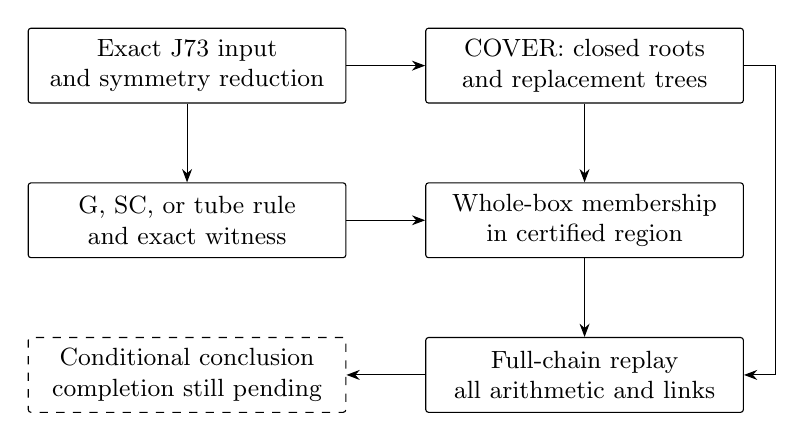
\begin{tikzpicture}[>=Stealth,font=\small,
 box/.style={draw,rounded corners=1pt,align=center,text width=3.8cm,minimum height=.95cm}]
 \node[box] (input) {Exact J73 input\\and symmetry reduction};
 \node[box,right=1cm of input] (root) {COVER: closed roots\\and replacement trees};
 \node[box,below=1cm of input] (local) {G, SC, or tube rule\\and exact witness};
 \node[box,right=1cm of local] (member) {Whole-box membership\\in certified region};
 \node[box,below=1cm of member] (replay) {Full-chain replay\\all arithmetic and links};
 \node[box,left=1cm of replay,dashed] (gate) {Conditional conclusion\\completion still pending};
 \draw[->] (input)--(root);
 \draw[->] (input)--(local);
 \draw[->] (root)--(member);
 \draw[->] (local)--(member);
 \draw[->] (member)--(replay);
 \draw[->] (root.east)--++(.4,0)|-(replay.east);
 \draw[->] (replay)--(gate);
\end{tikzpicture}
\caption{The proof obligations and the four certificate categories. Local
acceptance includes whole-box membership. Full-chain replay and the
dashed conditional conclusion remain unfinished.}
\label{fig:proofmap}
\end{figure}


\begin{samepage}
\section{The computation}\label{sec:computation}

\subsection{Initial grid and replacement trees}
The initial rational overcover uses a proved rational upper bound
$q_+>\pi$, obtained with a Machin formula and alternating-series bounds.
The rectangle
\[
 [0,2q_+/5]\times[0,q_+/2]\times[0,2q_+/5]\times[0,q_+/2]
                                  \times[-q_+/2,q_+/2]
\]
is split into $12\times17\times12\times17\times30=1{,}248{,}480$
rational atoms. The root order is part of the input declaration. Stored
binary64 boxes round outward from these atoms, so they form an
overcover and may overlap in positive volume. Within a replacement tree,
the exact cuts reconstruct the parent union \cite{input,verifier}.
\end{samepage}

The first traversal finished, but left unresolved roots. Its reported
48,895,305 accepted leaves are a historical producer count, not a final
arithmetic verification result \cite{map}. Later queues replace only the
unresolved leaves. Subdivision followed by certification of some children
can increase the number of unresolved leaves while reducing the region
they cover. We therefore distinguish original roots,
replacement inputs, terminal leaves, and pending tasks. None of their
count ratios measures the remaining geometric volume or difficulty.

The production search uses finite-time budgets, checkpointed trees, and
successive follow-up stages. The engine and storage format have changed
during the run. Checksums are computed from the decompressed certificate
data, so they do not depend on the compression format \cite{operations}.
Exceptions, time limits, unvisited stack entries, and
inconclusive signs all remain unresolved regions.

\section{Interim results}\label{sec:interim}

\subsection{Frozen production status}
The release snapshot was captured on 27 October 2026,
10:40:50.233026--10:41:21.245658 KST, without interrupting production.
Each root's committed logical proof was read through the compact-storage
API with read-only database connections. This is a rolling capture of
individual committed versions, not an atomic filesystem snapshot. The
coordinator counts and state were unchanged across capture, although its
progress heartbeat changed. The snapshot's per-root times and logical
SHA-256 digests are retained in \file{data/status-snapshot/}.

\begin{table}[ht]
\centering\small
\caption{Production counters in the frozen release snapshot. These are
not exhaustive independent verification results.}
\label{tab:counts}
\begin{tabular}{@{}p{.65\textwidth}r@{}}
\toprule
Quantity & Count\\
\midrule
Staged input jobs & 2,057\\
Closed staged jobs & 453\\
Open staged jobs & 1,604\\
Pending boxes in captured open proofs & 397,906\\
Closed receipts without a tube operation & 409\\
Closed receipts containing a tube operation & 44\\
Closed before coordinator stage 2 & 392\\
Additional closures by capture & 61\\
Coordinator stage-2 visits recorded & 136 / 1,665\\
\bottomrule
\end{tabular}
\end{table}

Here ``closed'' means closed in the production records. A tube-assisted
job contains at least one tube operation and may also contain $G$, $SC$,
or $COVER$ steps; these counts have not been verified by a full-chain
replay.

The recorded proof budget and the time at which a job closed are different
stage notions. Grouping the captured proofs by their recorded budget
gives 431 closed and 1,523 open at stage 1, and 22 closed and 81 open at
stage 2. The stage-1 closed receipts comprise 392 without and 39 with a
tube operation; stage 2 comprises 17 without and 5 with a tube operation.
Tube-only visits can retain an earlier budget, so these figures are not a
second chronology of stage closures. Likewise the coordinator's
136 visits are not 136 closures.

The exact summary bytes are identified by SHA-256
\begin{center}\small
\path{145d4f6cd74f64b01a0166dbc548a0121f92c87c45a29fbacfd814116c10dbf3}.
\end{center}
The manifest also binds the open-job list, compressed per-job status,
public capture records, source evidence, logical proof-version hashes,
and selected-certificate provenance. The raw controller record is not
distributed; the summary retains its original capture digest as
provenance. Production continues after this capture; later counters are
not substituted into this version.

\subsection{From the original grid to the staged jobs}
The original grid contains 1,248,480 angle roots. Its first traversal
reported 1,247,167 closed roots and 1,313 roots with 67,011 unresolved
descendant leaves. These are different units. A subsequent traversal
processed 32,420 leaf tasks and left 34,591 unprocessed. Subdivision of
the processed tasks produced 1,133,950 unresolved leaves, so the switched
queue had $1,133,950+34,591=1,168,541$ inputs. Its later unresolved-output
counts were
\[
\begin{split}
1,168,541&\longrightarrow244,200\longrightarrow36,895
\longrightarrow32,332\\
&\longrightarrow22,053\longrightarrow4,759
\longrightarrow4,105\longrightarrow3,524.
\end{split}
\]
These transitions replace unresolved output populations rather than
counts of original roots. In the transition from 32,332 inputs, 19,666
input jobs closed, leaving 12,666 input jobs whose unresolved descendants
numbered 22,053. Thus subtracting closed inputs does not give the
output-leaf count.

The later static ledgers partition those 3,524 residual jobs as follows:
\[
\begin{split}
3,524-15-25-1,401&=2,083,\\
2,083-1&=2,082,\\
2,082-4-21&=2,057.
\end{split}
\]
The first three reductions remove 15, 25, and 1,401 jobs. A separately
recorded closure of job 2411 leaves 2,082; removing another 4 and 21 jobs
gives the staged population of 2,057. The accompanying accounting table
identifies these disjoint sets. This checks the ledger, not the underlying
certificates.


\subsection{Tube closures and the remaining frontier}
The earlier tube study used a different frozen rolling snapshot, captured
on 26 October 2026, 10:25:18.766258--10:25:49.262151 KST. Among its
1,662 open staged jobs and 358,906 pending boxes, the verified region
union covered 7,450 boxes and every pending box of 39 jobs. The
independent review and subsequent checker record checked the 1,365 tube
applications in those complete frontiers \cite{tubefrontier}. This is a
local frontier result; it does not replay all earlier source, $G$, or
$SC$ witnesses for 39 original-grid roots. These historical counts are
not added to the current 44 tube-assisted producer receipts.

A tube certificate combines a local exclusion theorem with a whole-box
membership test. The contact-facet theorem permits any exact proper
reference rotation for which the stated support, positive torque-span,
and remainder conditions can be verified. Symmetry transport must use a
proper symmetry of J73 and must transport the viewing region as well.
The canonical mixed theorem covers its specified intersection; translating
that model to an arbitrary apparent coincidence is not justified.

Round~8 examined the remaining frontier by family, depth, and exact
scale-one witnesses. Numerical proximity to a catalogue rotation is a
candidate label, not a proof of an exact coincidence in the box. Conversely,
a box labelled ``none'' has not been proved disjoint from all coincidence
families. The frozen diagnostic tables and their times are given below;
they are distinct from the current production counters.

The round~8 diagnostic is the rolling snapshot captured on
27 October 2026, 01:16:44--01:17:26 KST. It contained 1,615 open staged
roots and 370,364 pending boxes. These historical counts are not the
current counters in Table~\ref{tab:counts}. Its source records and
SHA-256 digests are retained with the release provenance.

\begin{table}[ht]
\centering\small
\caption{Historical round~8 frontier: numerical family labels and
rigorous scale-one witnesses.}
\label{tab:frontier-family}
\begin{tabular}{@{}lrrr@{}}
\toprule
Label & Open boxes & Roots met & $\lambda=1$ boxes\\
\midrule
T & 55,032 & 558 & 3,596\\
D5 & 27,666 & 250 & 0\\
H1 & 38,082 & 243 & 0\\
CT & 50,593 & 203 & 0\\
TC & 11,295 & 137 & 0\\
H4 & 2,555 & 54 & 0\\
identity & 5,452 & 267 & 5,452\\
other & 16,142 & 178 & 0\\
none & 163,547 & 935 & 2,122\\
\midrule
Total boxes & 370,364 & & 11,170\\
\bottomrule
\end{tabular}
\end{table}

The family label uses the closer of the two screen lifts and the nearest
catalogue rotation at the box midpoint, with a cutoff of $0.01$ radians;
exact identity intersections take precedence. The labels $T,D5,H1,CT,TC,H4$
are names in that fixed catalogue, ``other'' collects its remaining
families, and ``none'' means outside the cutoff. The box classes are
disjoint, but one root can meet several classes, so the root column
cannot be added. These midpoint labels do not certify incidence. In
particular, 2,122 boxes labelled ``none'' have rigorous $T$ witnesses.

\begin{table}[ht]
\centering\small
\caption{Depth in the same historical round~8 snapshot.}
\label{tab:frontier-depth}
\begin{tabular}{@{}lrrr@{}}
\toprule
Depth & Open boxes & Roots met & $\lambda=1$ boxes\\
\midrule
0--9 & 289,143 & 1,348 & 9,043\\
10--19 & 79,239 & 580 & 2,092\\
20--29 & 1,650 & 29 & 35\\
30 & 332 & 23 & 0\\
\bottomrule
\end{tabular}
\end{table}

The rigorous witnesses establish scale one in 11,170 boxes of 577 roots:
5,452 identity boxes and 5,718 $T$ boxes. The identity and $T$ root counts,
267 and 316, overlap. Identity witnesses use exact rational
intersections. The nonidentity witnesses use a rational outer angle,
an outward-rounded inverse-frame enclosure inside the original box,
and exact symmetry or rigorous common-hull support inequalities giving
equality of the complete shadows. A catalogue match alone is insufficient.
The other 359,194 boxes are unclassified with respect to existence of a
scale-one point; no rigorous negative census was completed. Each reported
positive witness passed its construction or recovery check. The later
separate cross-check repeated every identity witness and a sample of
120 $T$ witnesses, rather than a second exhaustive replay of the latter.
This release includes the historical summaries and source hashes, but
omits the 3,304,005-byte witness file. Its format is not supported by the
exclusion checker, and the historical equality witnesses were not
replayed for this release.

All pending boxes of the 23 roots in the depth-30 row were at that depth.
Their small widths do not close their roots. Reapplying an unchanged
depth-limited search does not by itself resolve them. The diagnostic
studies found some additional finite tube covers in private copies, but
those covers were not production commits or independent acceptances of
the complete original-grid chain, and are not added to the production
closure counter here.


The remaining roots present several different obstacles. Some boxes meet
an exact equality family, so a strictly positive support gap is impossible
there. Signed-contact certificates allow a nonnegative sum, but the
required exact cancellations and nonnegative polynomial decomposition
still have to be found. A polynomial with an interior zero set need not
admit a finite proof by nonnegative Bernstein coefficients on axis-aligned
boxes in the existing coordinates. Some product enclosures also include
unreachable configurations; retaining the original-angle correlations or
constructively subdividing the cover can then matter more than increasing
precision.

Other roots have large shallow boxes, varying support sets, or weak
first-order torque span. A contact region can be valid yet fail to contain
the entire original angle box. Near an intersection of equality branches,
a uniform positive first-order bound can fail and a mixed estimate is
needed. Some production leaves have reached the present subdivision
depth; more elapsed search time alone does not create a new proof for
such a leaf. None of these observations proves that a passage exists or
that no certificate can be found. No completion date can be given.

\section{Verification and the trust base}\label{sec:verification}

\subsection{Checks required for the final claim}
The checker must reconstruct $V$, its ordering, central symmetry, the
group permutations, and the initial rational cover. It must then follow
every retained old leaf and every replacement, rebuild every split,
check closed boundaries, and recompute each accepted inequality and
membership test. A hash identifies the data to check; it does not prove
the inequality. Saved margins and PASS strings are not accepted as
mathematical evidence.

Earlier audits have different scopes. The historical source inventory,
recorded on 27 October 2026, reports two early samples of 40 and 60 $G$
witnesses. Later traversals replayed their own certificate populations
exhaustively, but did not certify the complete original-to-final chain
\cite{map}. The public accounting table in
\file{data/historical-accounting.md} identifies the replacement
populations. Exhaustive verification of a later traversal does not verify
certificates retained from earlier stages. Atlas checks likewise establish
their local regions and recorded applications, not coverage of all
unresolved roots. The final replay must include both the retained
first-pass witnesses and every adopted follow-up witness.

The release replay checks three local certificates (a $G$ leaf, an
$SC$-based closed fan cover, and a $tube$ application) and all 2,660
regions. It does not check the complete history of any original-grid
root. The final verification must include every original root and adopted
replacement, with no missing or unresolved region.

\subsection{Arithmetic and independence}
Exact contact identities use rational arithmetic and ordered
$\Q(\sqrt5)$ comparisons. New certificate inputs must use integers,
canonical rational strings, or exact coefficient pairs; Boolean and
floating-point inputs must be rejected. Legacy binary64 endpoints must
be interpreted as the
exact rationals represented by their stored bits, retaining the whole
declared box.

Radicals, trigonometric functions, and coordinate maps require outward
enclosures. Existing paths use Fraction-based rational bounds and
Taylor remainders, or python-flint with FLINT/Arb. A working precision
such as 320 bits is not itself a proof of a sign. An interval crossing
zero does not prove nonnegativity; an exact zero identity does.
Inconclusive comparisons must be rejected or kept unresolved.

The ordinary verifier is implemented separately from the producer
\cite{verifier}, but the singular and newer local checkers share some
geometry and arithmetic modules. The trust base includes the
stated mathematical reductions and exclusion theorems, their checker
implementations, parsing and cover reconstruction, integer and interval
arithmetic, the interpreter and libraries, and execution on the recorded
hardware. Formal proof-assistant verification of the complete J73 chain
has not been supplied.

Candidate hulls, numerical optimization, linear programs, scheduling, and
language-model output need not be trusted if all their witnesses are
rechecked by the stated exact predicates. The discovery checker uses
Python assertions. Run all checks without \file{-O} or
\file{PYTHONOPTIMIZE}; \file{self_test.py} rejects optimized execution.

The included checker source files, their hashes, and the measured release
checks are listed in the repository. Appendix~\ref{app:release} separates
this local test scope from the unfinished full-chain verification.

\section{Limitations}

The global exclusion remains unfinished. The frontier obstacles and the
scope of the local estimates are described in Section~\ref{sec:interim}.
Neither the contact-patch nor the signed-contact theorem has been shown
to replace every legacy witness in the retained chain. A complete result
still requires the dependencies and full-chain checks of
Section~\ref{sec:verification}.

Private historical source records are identified as not distributed in
\file{paper/SOURCES.md}. No conclusion about J74 or J75 is drawn from
this work.

\section{Data and code availability}

The accompanying repository contains the certificates and omissions
listed in \file{README.md}. Its self-test checks the included local
evidence, file hashes, and PDF page count. The software archive is
\authorconfirm{version-specific DOI}; the repository is
\url{https://github.com/ysmin1575/j73-rupert}. The preprint DOI is
\authorconfirm{paper DOI reserved for the separate preprint}.

The program and exact data for Section~\ref{sec:hidden} are included in
\file{code/discovery/}. The program reconstructs the vertices, rotations,
sign comparisons, orbit, pose labels, and four-contact identities without
importing production modules.

A future complete archive must additionally bind every original root,
every adopted replacement, all retained old witnesses, and the complete
verification result. The present sample or staged population does not
supply that archive. The source-to-claim map for the mathematical text is
\file{paper/SOURCES.md}.

The producer derives from Gihyo Jung's MIT-licensed project
\cite{jung}, pinned in the input record at
\file{2b45714fc243c320bd9c6bae00257835755af040}. Its attribution and full
MIT notice are retained in the accompanying \file{NOTICE}. Code is
released under the MIT license. The paper text and data are released
under CC BY 4.0; this does not relicense upstream code.

\begin{samepage}
\section{AI-use statement}

Claude (Anthropic) and OpenAI Codex assisted with literature checks,
mathematical derivations, code, and drafting. Mathematical acceptance
requires the stated exact or outward-rounded checks rather than a
language-model response. The author directed the project and takes responsibility for the submitted text.
Verification of the complete certificate chain remains unfinished.
\end{samepage}

\appendix
\section{Release scope and outstanding verification}\label{app:release}

The release runtime uses $G$, $SC$, $COVER$, and $tube$. The exact
parser, arithmetic, geometry, polynomial evidence, coordinate images,
local rules, and closed-cover reconstruction belong to its trust base.
The exporter, search heuristics, and stored producer verdicts do not.
These boundaries are documented with the checker sources and digest
manifest. The discovery program is independent of that runtime and of the
producer.

Conversion of all legacy production witnesses remains in progress. The
final version will give a migration record for every replaced leaf,
including its unchanged parent region and whole-box membership. Until
that replay succeeds, the original witness and its original proof
dependencies cannot be discarded. A partial local receipt cannot be
promoted to a complete-root or complete-grid verdict.

Only the software version DOI, software concept DOI, and paper DOI remain
open for confirmation at upload. The software concept DOI is recorded
separately in the repository README.

\begin{thebibliography}{99}
\raggedright
\bibitem{sy} J. Steininger and S. Yurkevich,
\emph{A convex polyhedron without Rupert's property},
\href{https://arxiv.org/abs/2508.18475v2}{arXiv:2508.18475v2},
28 January 2026. In particular, Theorems 17 and 36.

\bibitem{algorithmic} J. Steininger and S. Yurkevich,
\emph{An algorithmic approach to Rupert's problem},
Math. Comp. 92 (2023), 1905--1929.
\href{https://doi.org/10.1090/mcom/3831}{doi:10.1090/mcom/3831};
\href{https://arxiv.org/abs/2112.13754v2}{arXiv:2112.13754v2}.

\bibitem{fredriksson} A. Fredriksson,
\emph{Optimizing for the Rupert property},
Amer. Math. Monthly 131 (2024), 255--261;
\href{https://arxiv.org/abs/2210.00601v2}{arXiv:2210.00601v2}.

\bibitem{gg} R. Gosain and B. Grimmer,
\emph{Some New Insights from Highly Optimized Polyhedral Passages},
\href{https://arxiv.org/abs/2509.08190v1}{arXiv:2509.08190v1},
9 September 2025, especially Table 4.

\bibitem{lw} \texttt{L, W} (registered creator name),
\emph{The Snub Cube and Snub Dodecahedron Are Not Rupert},
preprint, 3 October 2026.
\href{https://doi.org/10.5281/zenodo.23118432}{doi:10.5281/zenodo.23118432}.

\bibitem{jung} G. Jung,
\emph{The rhombicosidodecahedron is not Rupert},
preprint, 5 October 2026.
\href{https://doi.org/10.5281/zenodo.23159625}{doi:10.5281/zenodo.23159625}.
Code: \url{https://github.com/swiri0921-bit/rhombicosidodecahedron-not-rupert}.

\bibitem{hervay} B. Hervay,
\emph{Non-Rupertness of the Rhombicosidodecahedron},
preprint, 28 September 2026.
\href{https://doi.org/10.5281/zenodo.23013945}{doi:10.5281/zenodo.23013945}.

\bibitem{murphy} T. Murphy VII (Tom 7),
\emph{Noperts}, source repository and verification notes,
\url{https://github.com/tom7/noperts}, particularly
\texttt{snub-cube.md} and \texttt{snub-dodecahedron.md}.
Accessed 25 October 2026.

\bibitem{yoo} S. Yoo,
\emph{On the touching arc of the snub cube: a closed form and an
independent check}, 15 October 2026.
\href{https://doi.org/10.5281/zenodo.23397416}{doi:10.5281/zenodo.23397416}.

\bibitem{input} J73 release documentation,
\emph{Exact input and D5 reduction}, Section~\ref{sec:body} and
Section~\ref{sec:computation} of this report; accompanying
\file{code/checker/geometry.py} and
\file{data/status-snapshot/release-input-binding.json}.
The complete original-root cover is not replayed by this release.

\bibitem{hidden} S. Yoo, exact discovery data and independent check,
incorporated in Section~\ref{sec:hidden}; accompanying
\file{code/discovery/check.py} and \file{code/discovery/evidence.json}.
The discovery note is not issued separately with this release.

\bibitem{patch} J73 release documentation,
\emph{Uniform contact-patch theorem}, Theorem~\ref{thm:patch}
of this report; contact-facet checking in the accompanying
\file{code/checker/tube.py}.

\bibitem{signed} J73 release documentation,
\emph{Signed-contact theorem and exact polynomial certificates},
Theorem~\ref{thm:signed} of this report; accompanying
\file{code/checker/local.py} and \file{code/checker/polynomial.py}.

\bibitem{fan} J73 release documentation,
\emph{Closed fan polygons and rotation cones},
Section~\ref{sec:fan} of this report; accompanying
\file{code/checker/cover.py}.

\bibitem{tube} J73 release documentation,
\emph{Canonical mixed-barrier tube and region certificates},
Section~\ref{sec:tube} of this report; accompanying
\file{code/checker/tube_intersection.py} and
\file{data/tube-regions.json}.

\bibitem{review} J73 historical verification records,
\emph{Mixed-barrier estimates and whole-box containment},
private records, not distributed; provenance inventory dated
27 October 2026. Source IDs \file{src-cbdc118ba294b922} and
\file{src-917e39759c5a7705}; their full SHA-256 digests and byte sizes
are recorded in the accompanying \file{paper/SOURCES.md}.
The corrected arguments are in Sections~\ref{sec:tube}
and \ref{sec:membership} of this report.

\bibitem{membership} J73 release documentation,
\emph{Whole-box membership and coordinate connection},
Section~\ref{sec:membership} of this report; accompanying
\file{code/checker/image.py}, \file{code/checker/tube.py}
and \file{code/checker/cover.py}.

\bibitem{map} J73 historical source inventory,
\emph{Proof map, certificate inventory, and trust base},
private records, not distributed; provenance inventory dated
27 October 2026. Source IDs \file{src-fdc77b2b3dd84f4c},
\file{src-14c86cbed8f0f001} and \file{src-ca6e021cfc12af91};
their full SHA-256 digests and byte sizes are recorded in
\file{paper/SOURCES.md} and \file{data/source-evidence-manifest.json}.
These historical records are not final production statistics.

\bibitem{legacy} J73 release documentation,
\emph{Retained legacy proof obligations},
Sections~\ref{sec:interface} and \ref{sec:verification} of this report;
accompanying \file{PROOF_MAP.md}.
The historical balls, tapers and collision arguments remain dependencies
where retained witnesses use them; their complete payloads and
original-to-final replay are not supplied by this release.

\bibitem{tubefrontier} J73 historical diagnostic summary,
\emph{Tube-frontier coverage for the snapshot of 26 October 2026
and independent verification}, accompanying
\file{data/historical-diagnosis/README.md} and its provenance in
\file{data/status-snapshot/historical-diagnosis-manifest.json}.
The counts concern the captured pending frontiers, not an end-to-end
acceptance of original-grid roots.

\bibitem{verifier} J73 release documentation,
\emph{Independent J73 checker, version 2}, accompanying
\file{code/checker/}. The release README and self-test record state
its tested population; no complete-grid acceptance is asserted.

\bibitem{operations} J73 historical accounting and frozen status,
\emph{Production counters, root partitions, and provenance},
accompanying \file{data/status-snapshot/}, its SHA-256 manifest,
and \file{data/historical-accounting.md}.
The source-to-claim map is \file{paper/SOURCES.md}.
These are production counters and ledger checks, not exhaustive
verification results.
\end{thebibliography}

\end{document}
